%!TEX root = ../document.tex
\chapter{绪论}
\section{研究背景与意义}

我国经过二十余年的信息化建设,互联网用户仍在持续增长,根据中国互联网信息中心发布的第43次《中国互联网络发展%
状况统计报告》\upcite{43CNNIC}显示,截止2018年12月,我国网民规模达8.29亿,较2017年末仍增加了3.8\%,互联%
网普及率达59.6\%,其中移动互联网用户比例更是高达98.6\%。
浩如烟海的数据填充着互联网,人们要从海量数据中找到自己关心的部分变得越来越难。
推荐系统是帮助用户从海量产品集合里面找到感兴趣目标的软件应用,具有千人千面的特点,也是数据挖掘和机器学习%
相关科技在实践领域最成功的应用之一。
在许多网站和应用程序中,例如电子商务、新闻和视频网站、%
音乐和广播电台等,他们都需要为用户推荐可能喜欢物品的杰出服务,如今接收不同形式的自动推荐已经成为我们日常%
在线用户体验的一部分。在典型的在线网站上面,可以收集用户各种类型的相关动作,例如:用户点击、浏览、收藏、购买%
了某个商品。
推荐系统(RS)已发展成为帮助用户做出明智决策和选择的基本工具,尤其是在大数据时代,%
客户必须从大量产品和服务中做出选择。因此现代推荐系统是在当前大数据环境下应运而生的,%
现代推荐系统的架构如图\ref{fig:RS_Architecture}所示,本文讨论的问题主要出于推荐算法层面。

\begin{figure}[htb]
  \centering
  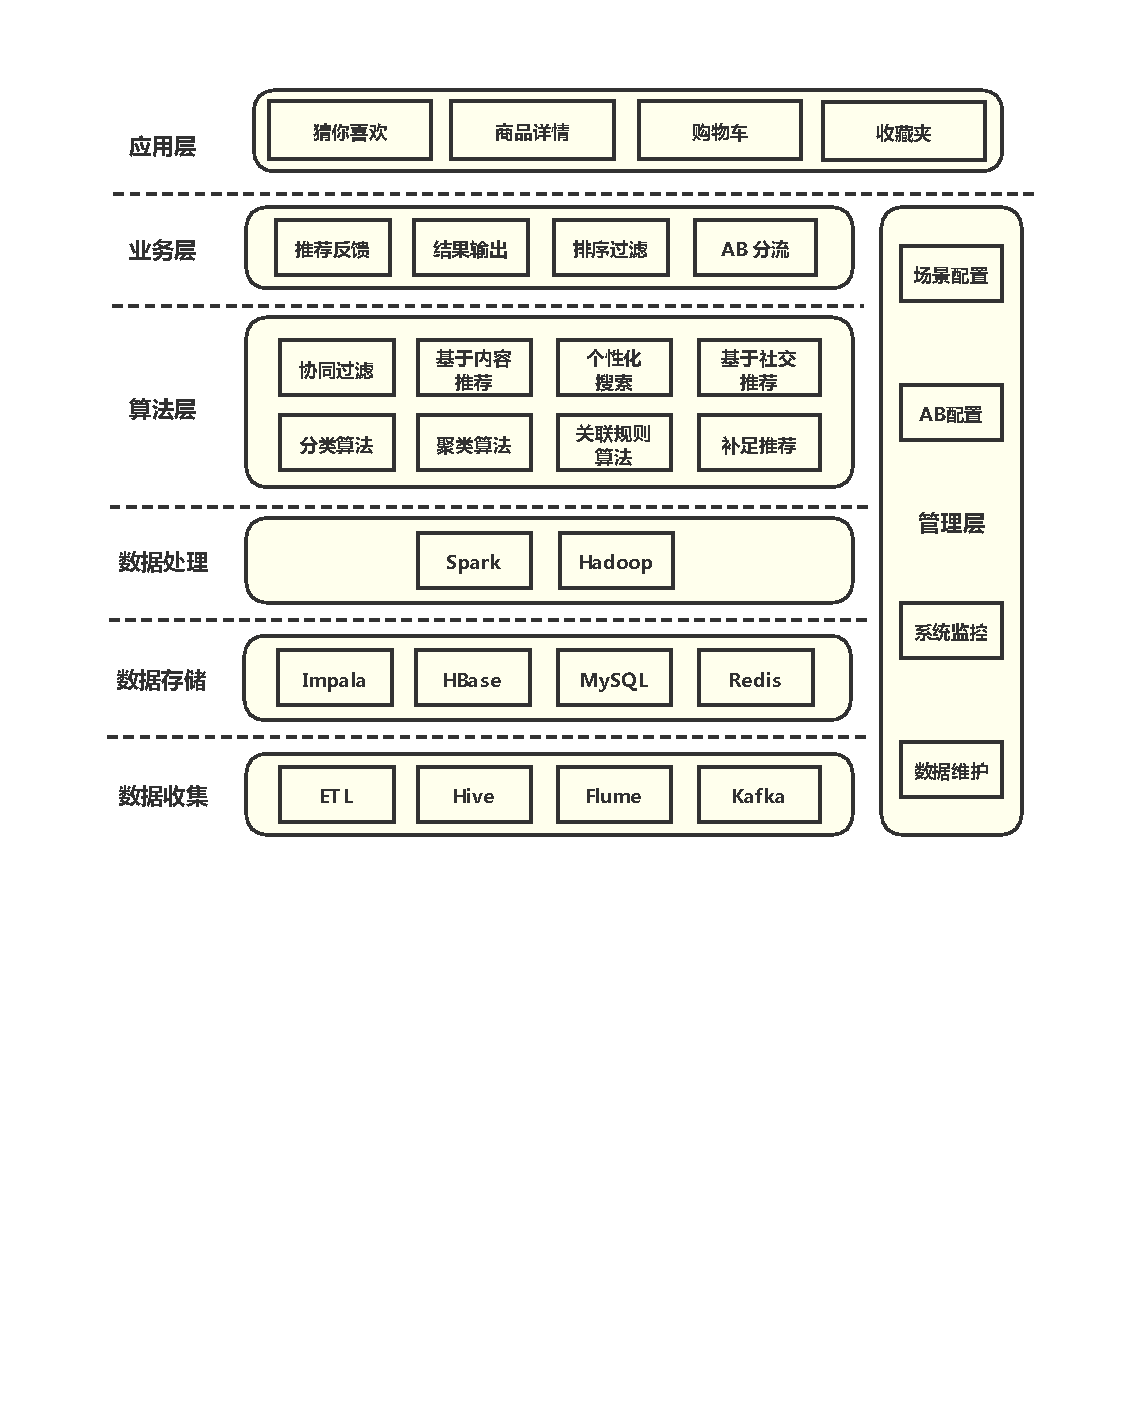
\includegraphics[width=\linewidth]{RS_Architecture.pdf}\\
  \caption{现代推荐系统架构图}
  \label{fig:RS_Architecture}
\end{figure}
推荐算法作为推荐系统的灵魂,承担着推荐高品质项目和高效反馈的重任,因此设计鲁棒性好的推荐算法有着重要的研究意义。
现有的推荐策略都主要关注如何为用户或项目找到临近集,或者利用其它的显式或隐式信息(如标签、评论、%
项目属性和用户个人信息)来提升近邻感知能力。然而,这些静态算法都没有考虑用户兴趣变化的实时动态性。时序信息%
就是反应用户兴趣实时变化的一个重要特征,在许多任务比如用户下一行为预测中,用户下一首会听什么歌与用户的%
喜好、当前所处环境的上下文都高度相关。

推荐系统面对的任务主要有两部分:评分预测和产品推荐。所以根据用户的历史%
记录预测他下一次会选择什么也是推荐领域一个严峻的挑战。

% 推荐系统面临的另外一个巨大挑战就是处理新用户和新物品,也就是所谓的冷启动问题,因为这些用户/物品的特征在缺少数据时很难正确判断。近来,迁移学习\upcite{YangTransfer}被用于解决推荐系统的冷启动问题。迁移学习通过利用辅助域来在目标域上获得提升


因此本文提出序列建模的推荐思路,本文的研究内容是结合神经网络的序列建模技术和推荐系统相关理论知识,实现快速向用户推荐可能感兴趣的物品。%
充分利用深度神经网络强大的建模能力,提取用户行为的重要时序特征,构建推荐对象的兴趣模型,%
% 再结合迁移学习的泛化能力,
构建相关模型来识别用户的兴趣意图,综合考虑推荐对象和用户两者之间%
的特征信息挖掘两者之间的隐式联系,从而发掘出用户感兴趣的物品,
以此来帮助用户快速的找到有感兴趣的物品,提升网络应用的流量及用户的黏性。%

%
% 本章节主要从传统机器学习和深度学习两个方面介绍现代推荐系统中常用的各种推荐算法,%
% 从它们各自的特点分析现如今存在的问题。

\section{国内外研究现状}

为了分析和理解国内外现有推荐算法的各自特点,本章节根据其使用的技术不同分为两个大类分别进行描述,
同时给出了如图\ref{fig:RA_clsssification}的思维导图。

\begin{figure}[htb]
  \centering
  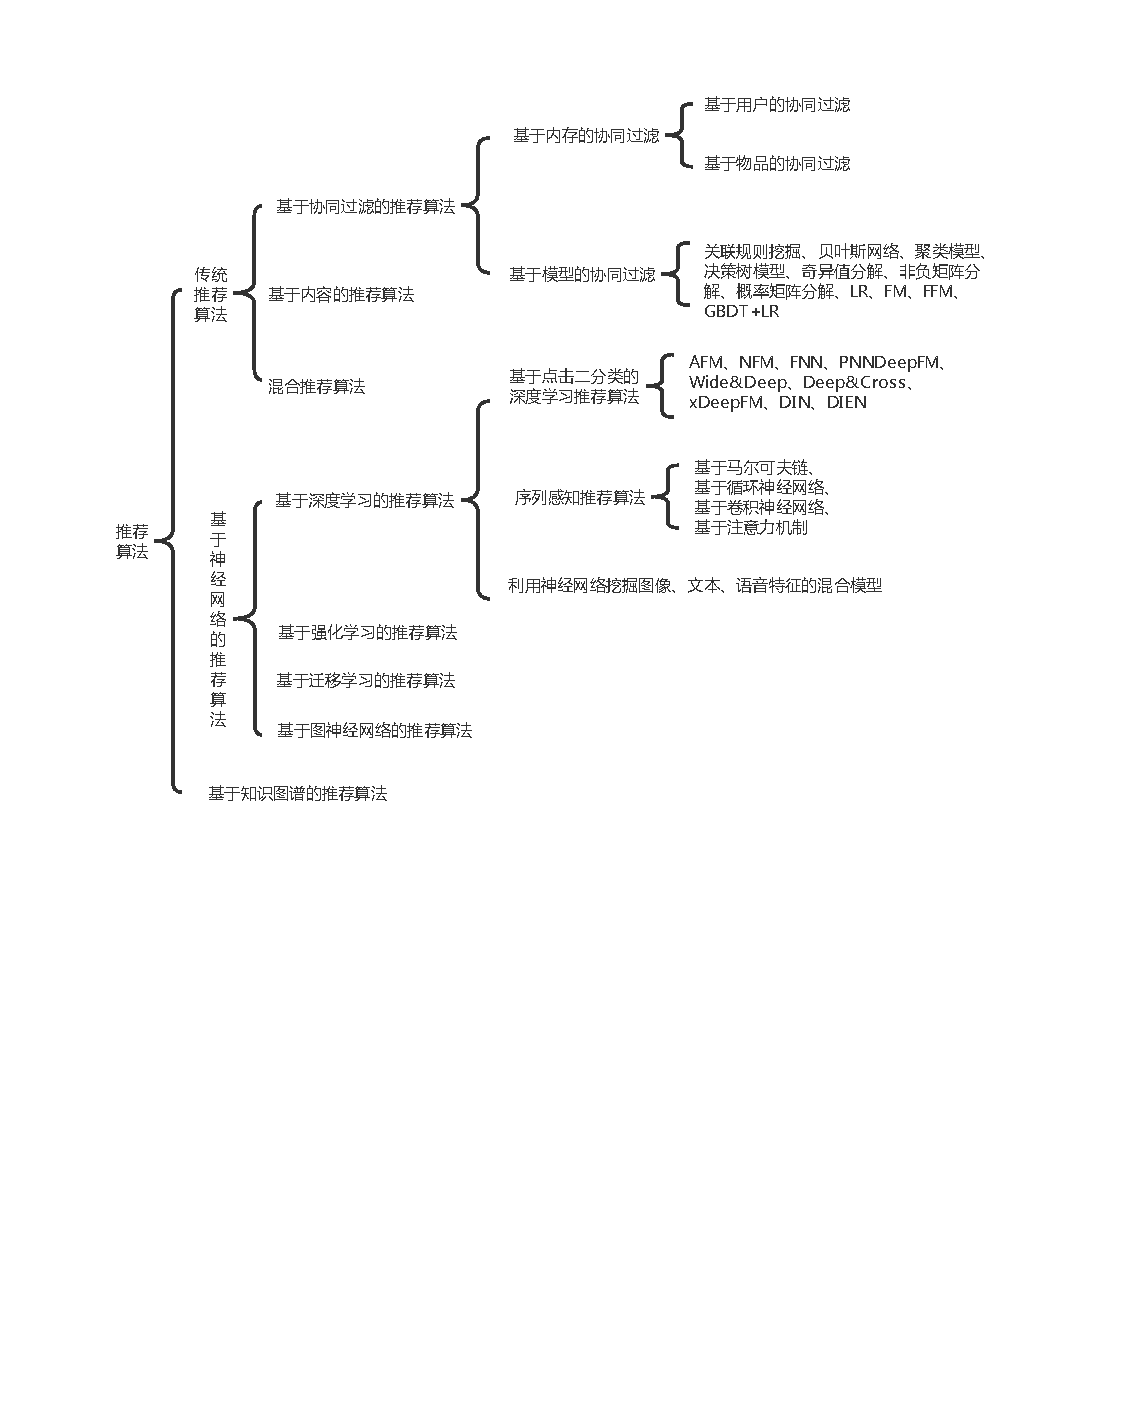
\includegraphics[width=\linewidth]{RA_clsssification.pdf}\\
  \caption{推荐算法分类思维导图}
  \label{fig:RA_clsssification}
\end{figure}

\subsection{传统推荐算法}

传统的经典推荐算法主要可分为三大类,它们分别是基于协同过滤的推荐算法、基于内容的%
推荐算法和混合推荐算法。协同过滤算法大体上可以分为基于内存的协同过滤(Memory-based CF)%
和基于模型的协同过滤(Model-based CF)。基于内存的协同过滤通过为用户寻找具有相似行为的用户%
或有相似特点的物品集合做推荐,所以可细分为基于用户的协同过滤%
(User-based Collaborative Filtering,UBCF)和基于物品的协同过滤%
(Item-based Collaborative Filtering,IBCF)。
而基于模型的协同过滤则主要利用评分信息训练相应的模型,然后使用这个模型对未知数据进行预测,%
这类算法有贝叶斯网络\upcite{chien1999bayesian}、聚类模型\upcite{ungar1998clustering}、%
概率矩阵分解\upcite{Salakhutdinov:2007:PMF:2981562.2981720}等等。
在基于内容的推荐算法中仅利用了单个用户的行为和数据给出对用户的推荐,特别是物品的描述和用户的属性描述在内容推荐中起到了关键作用。基于内容的
推荐精确度往往有限,还面临着严重的冷启动问题。
混合推荐系统则通过将上述两大类算法中的一个或多个结合起来以避免和克服某个单一算法带来的缺点。混合推荐算法中比较常见的方式是将基于内容的推荐方法与其他方法进行融合以避免冷启动、数据稀疏和扩展性等问题。
基于传统推荐算法的特点,%
基于协同过滤的推荐算法中大多需要构造一个用户与物品的交互矩阵,随着大数据的极速发展,%
物品与用户的数量往往能达到上亿规模,使得交互矩阵构造的空间复杂度过高,在大数据时代传统推荐算法已慢慢无法解决当%
前所面对的问题。

\subsection{基于深度学习的推荐算法}

得益于神经网络的反向传播理论,批量梯度下降的网络权重优化方式使得机器学习特别是深度学习%
能处理的数据规模没有理论上的数量限制,现代推荐算法也借助神经网络的技术蓬勃发展。%
神经网络领域下面子领域里的许多技术都已经被应用于推荐系统当中,包括深度学习、强化学习、迁移学习和图神经网络。%
本文仅讨论基于深度学习的推荐算法。

学术界推荐算法的发展离不开工业界的实践,而推荐算法在工业界的实践应用也为学术界的发展指引着方向。
推荐算法在工业界的一个重要实践就是进行点击率预估。随着深度学习技术被引入点击率预估方面,开始有大量的成果诞生。
点击率预估的通常做法是将推荐问题转化为二分类的有监督学习问题,算法建模的样本对象是物品,将用户的特征与物品特征拼接在一起构造高维样本,预测对象用户是否可能会点击目标物品。
在深度学习技术没有被引入点击率预估之前,传统做法通常使用逻辑回归\upcite{Kondakindi2014ALR}进行点击二分类,但这需要构造大量手工特征,FM\upcite{Rendle:2010:FM:1933307.1934620,Rendle:2012:FML:2168752.2168771}、FFM\upcite{Juan:2016:FFM:2959100.2959134}和GBDT+LR\upcite{He:2014:PLP:2648584.2648589}的出现让这类点击二分类模型能够自动学习到一些二维组合特征或者一些高维特征。随着深度学习的引入,特征的挖掘变得更加充分,组合特征的学习变得更加高效。

深层神经网络模型引入到点击二分类算法当中大多是通过神经网络与其他基础算法结合的方式构建混合模型,这些方法根据其网络融合的方式大致可以分为\textbf{串行融合}和\textbf{并行融合}两大部分。
\textbf{串行融合}的方式主要将FM等模型的输出作为MLP的输入,将FM视为交叉特征提取器,这类模型有:
Weinan Zhang等在 2016 年提出的因子分解机神经网络(Factorisation Machine supported Neural Network,FNN)\upcite{Zhang_2016},其将考FM与MLP进行了串联结合,利用FM为多层感知机MLP提取二维交叉特征进行点击率预估推荐;
Xiangnan He等在2017 年提出的神经网络因子分解机(Neural Factorization Machines,NFM)\upcite{He_2017}加入了池化层,将FM生成的二维交叉特征进行了元素级别的两两向量内积,引入了更多的非线性关系;
和Jun Xiao等人在2017年提出了注意力因子分解模型(Attentional Factorization Machine,AFM)\upcite{Xiao_2017},用注意力网络替换了上述两个模型中MLP,让Attention网络更好利用FM的二阶特征;Yanru Qu等人在2016年提出了基于向量积的神经网络(Product-based Neural Networks,PNN)\upcite{Qu_2016},与NFM不同的是使用了FM生成的二维交叉特征进行了元素级别的两两向量内积进行计算。
\begin{figure}[htb]
  \centering
  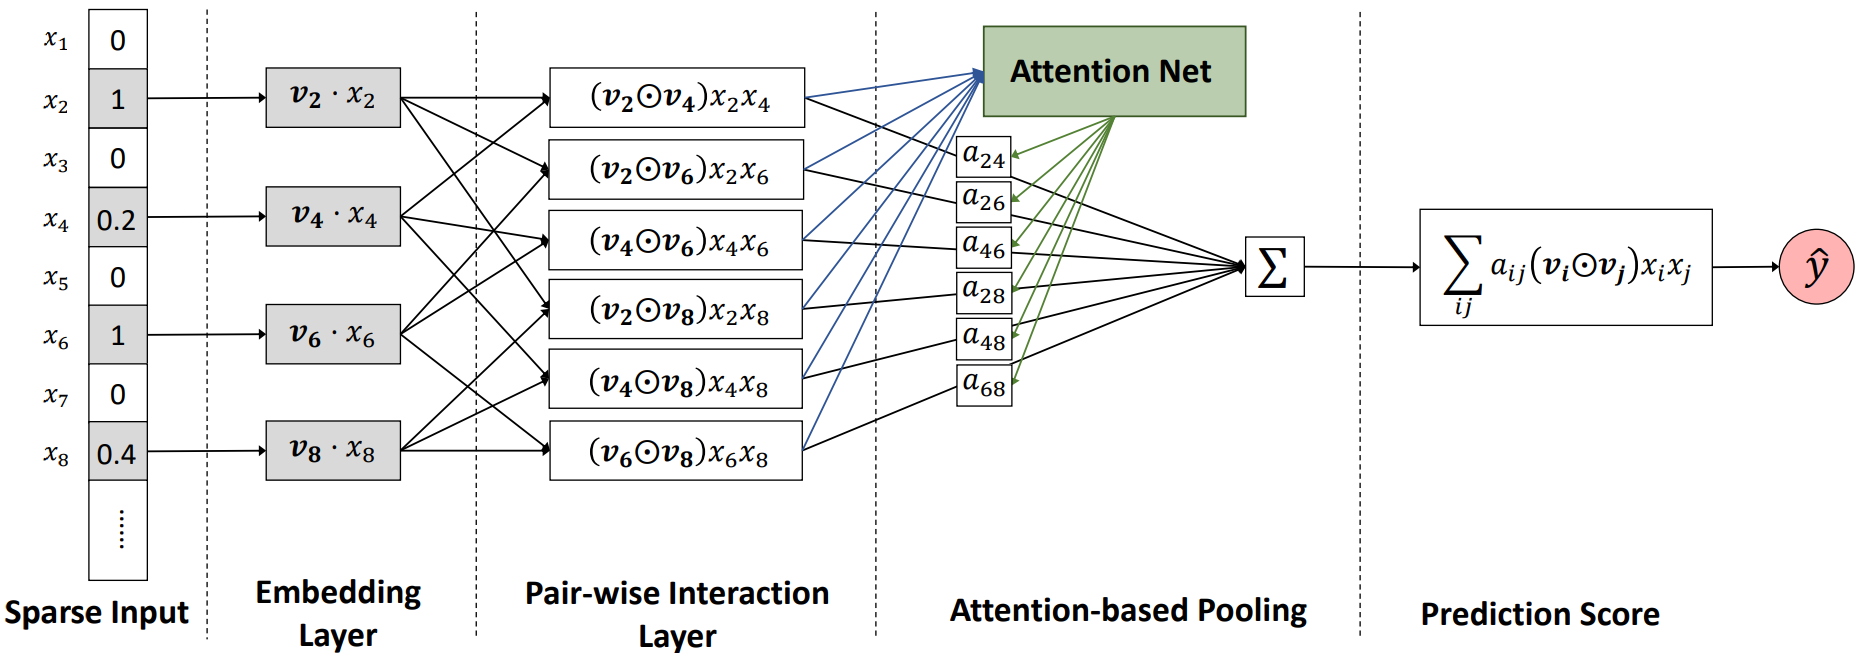
\includegraphics[width=\linewidth]{AFM.png}\\
  \caption{串行深度网络推荐模型之——AFM网络结构图\upcite{Xiao_2017}}
  \label{fig:AFM}
\end{figure}

而\textbf{并行融合}的方式则是利用两个或多个网络模块,每个子模块负责提取不同维度的特征为主要思路,构建点击二分类算法。这类模型主要有:


2017年Huifeng Guo等人将FM与MLP并行连接,提出的DeepFM模型\upcite{ijcai2017-239},两个组件网络共享同一个输入并行训练,能同时提取特征的低维和高维特征;
2016年Heng-Tze Cheng等人将一个Wide网络模型与深层网络Deep模型并行连接,利用Wide模块提升模型的记忆性,利用Deep模块提升模型的泛化性,构造的Wide\&Deep模型\upcite{Cheng_2016};
2017年Ruoxi Wang等人将深层网络Deep与一个交叉网络Cross并行连接,利用不同层数的Cross网络构造出任意维度的交叉特征,提出了Deep\&Cross模型\upcite{Wang:2017:DCN:3124749.3124754};
2018年Jianxun Lian等人提出了一个新颖的压缩交互网络(Compressed Interaction Network, CIN)的神经模型用于自动学习显式的高阶特征交互,然后将其与DNN模块并行集成,构造了一个名为极深因子分解机的模型(xDeepFM)\upcite{Lian:2018:XCE:3219819.3220023}用于同时以显式和隐式的方式自动学习高阶的特征交互。
\begin{figure}[htb]
  \centering
  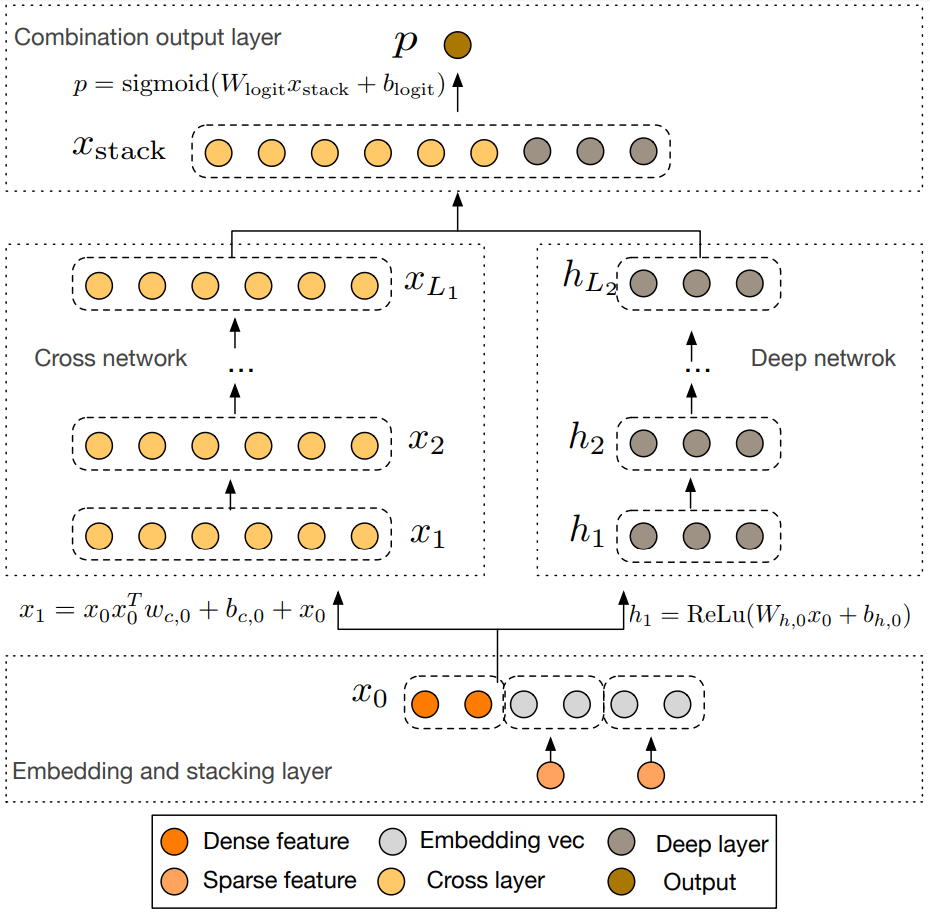
\includegraphics[width=0.7\linewidth]{Deep_Cross.png}\\
  \caption{并行深度网络推荐模型之——Deep\&Cross网络结构图\upcite{Wang:2017:DCN:3124749.3124754}}
  \label{fig:Deep_Cross}
\end{figure}
在串行模型与并行模型之外,又有一类\textbf{综合并行结构与串行的结构},如2018年Guorui Zhou等人先后提出了深度兴趣网络(Deep Interest Network,DIN)\upcite{Zhou:2018:DIN:3219819.3219823}和深度兴趣演化网络(Deep Interest Evolution Network ,DIEN)\upcite{zhou2018deep},DIN的并行结构体现在对用户侧历史行为特征域和物品侧特征域并行嵌入,堆叠组合成的向量再输入到全连接神经网络中去。DIEN对DIN的改进在于并行结构的特征嵌入部分考虑到了用户兴趣的演化进程,其使用双层GRU对用户历史行为的序列进行建模,将建模后的向量一起并入堆叠向量当中。

\subsection{序列感知推荐研究现状}

现有的推荐算法几乎很少有考虑到隐藏在用户历史行为序列中的用户兴趣动态变化情况,而且以上提到的基于深度学习的推荐算法都是以构造大量特征为基础进行建模的,这些算法都需要收集大量用户隐私数据,况且在某些特殊应用场景下,例如用户在使用在线服务但并未登陆或匿名的情况下,以构造大量特征为前提的算法将全部失效。考虑到这三类情况,本文提出了序列感知推荐算法,以用户历史行为组成的序列为数据进行建模推荐,无需使用大量用户隐私相关数据,在用户匿名状态下也可以根据当前服务的会话构成行为序列。
序列感知推荐算法许多学者称为基于会话的推荐算法,其中使用的序列建模算法基本可以分为RNN和CNN两大方向。在使用RNN进行序列建模推荐算法中,其中最广为人知的工作为2016年Balazs Hidasi等于提出的使用循环神经网络的基于会话的推荐算法GRU4Rec\upcite{DBLP:journals/corr/HidasiKBT15},首次通过使用循环神经网络利用会话的序列进行建模推荐,这类使用循环神经网络对序列进行建模进行推荐的还有Devooght等人于2017年提出的\upcite{devooght2016collaborative,Devooght:2017:LSR:3079628.3079670},Massimo等人\upcite{Quadrana:2017:PSR:3109859.3109896}在RNN的基础上利用Hierarchical RNN构建的序列感知推荐模型,2017年Yu Zhu等人在使用LSTM对序列建模的基础上加上了对时间间隔的考虑,提出了Time-LSTM模型\upcite{ijcai2017-504}。基于RNN的序列建模方法有较好的性能,但受固于RNN的递归结构,算法难以并行实现。
\begin{figure}[htb]
  \centering
  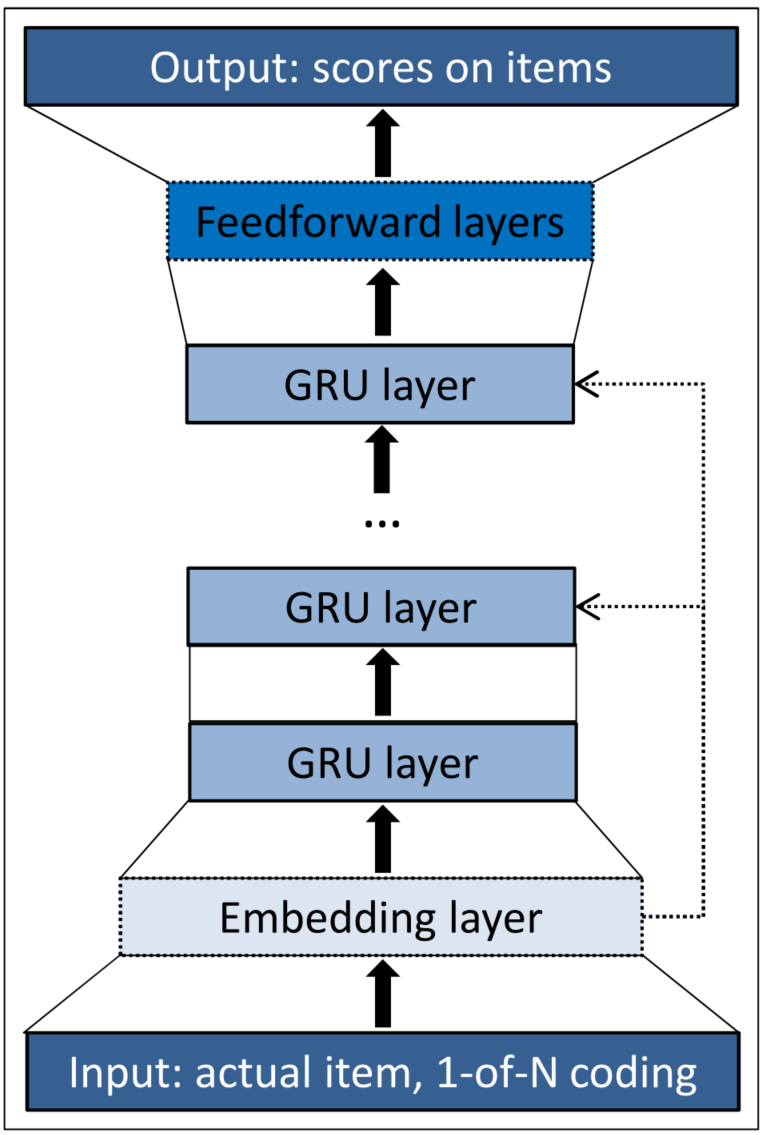
\includegraphics[height=7.5cm]{GRU4Rec.png}\\
  \caption{使用循环神经网络进行序列推荐算法之——GRU4Rec网络结构图\upcite{DBLP:journals/corr/HidasiKBT15}}
  \label{fig:GRU4Rec}
\end{figure}

另外一类序列感知推荐算法的方向是使用CNN对用户行为历史记录进行序列建模,CNN常用于计算机视觉领域图像特征提取,用于序列建模需要对基本的卷积结构进行大量的修改,这其中知名的工作有2018年Jiaxi Tang等人将序列嵌入矩阵使用CNN提取特征,提出的卷积序列嵌入推荐模型Caser\upcite{Tang:2018:PTS:3159652.3159656}。
\begin{figure}[htb]
  \centering
  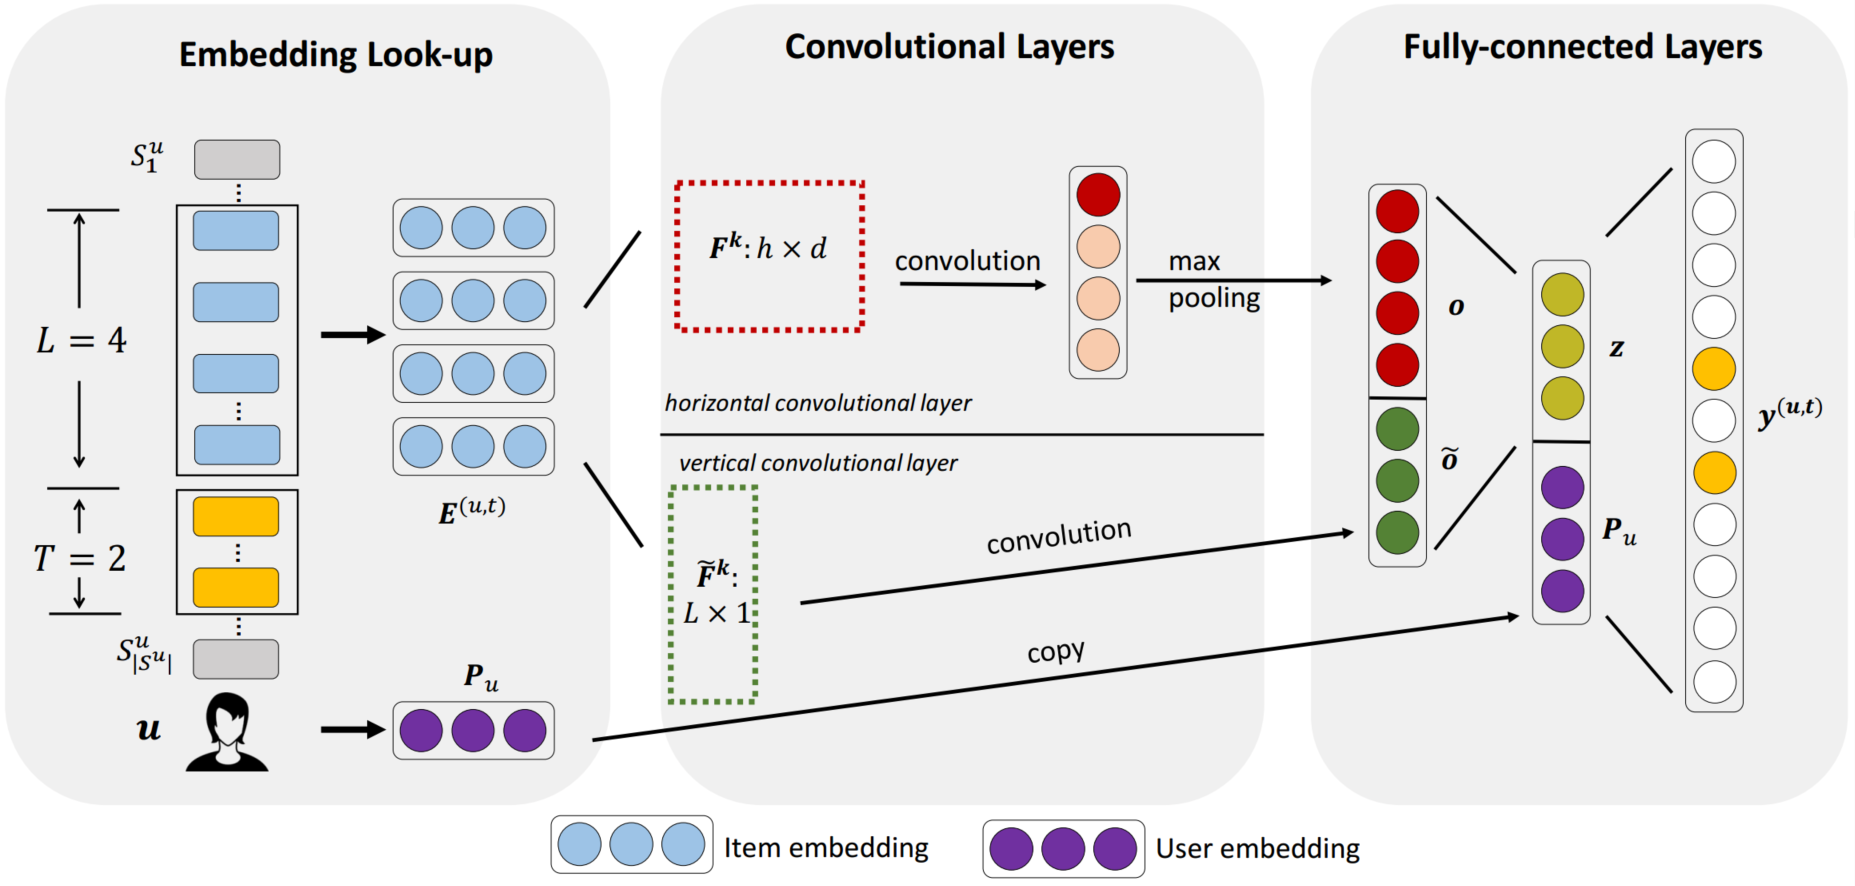
\includegraphics[width=\linewidth]{Caser.png}\\
  \caption{使用卷积神经网络进行序列推荐算法之——Caser网络结构图\upcite{Tang:2018:PTS:3159652.3159656}}
  \label{fig:Caser}
\end{figure}

基于CNN的序列建模方法适合抽取局部邻域特征,因此更适合短序列建模,如果要扩展记忆的序列长度则严重依赖卷积层的深度和感受野的大小,而这会显著增加计算量。

\section{研究内容和方法}
\subsection{研究内容}
本文通过调研分析国内外推荐算法的发展状况,特别是深度学习在推荐系统领域的发展情况,
分析了目前深度学习在解决推荐系统实际应用中遇到的挑战,本文提出了一种新的思路——序列建模,去解决推荐系统现有的问题,详细阐述了该序列感知推荐模型的工作步骤和方式。受神经网络在自然语言处理方面强大的建模能力,本文还提出了两种序列感知推荐模型。
最后本文通过对现实世界中两个数据集上进行的实验,对提出的模型进行了有效性验证。

\subsection{研究方法}
本文主要采用的研究方法有如下几点:
第一,文献调研法。通过互联网技术访问线上各个数据库中检索了大量研究领域的相关书籍、论文等学术成果%
,经过对国内外的相关研究文献与资料的全方位收集和分析,并结合工业界应用领域的最新解决方案,确立本文研究方向和主题,%
设计本文推荐模型框架及各模块之间的耦合。
第二,迁移法,本文是建立在自然语言处理、文本挖掘、推荐系统等相关技术的研究基础之上,通过综合%
探索以上技术理论,将其自然语言处理中的序列建模技术迁移到推荐系统的算法设计上来。
第三,实验仿真与分析法,本文通过调研和分析大量文献,提出本文的研究内容,为了验证本文提出的模型的%
有效性,本文在多个真实的数据上进行了实验,从而检验模型的可靠性。

\section{本文主要贡献}
本文通过前期大量文献调研,对比国内外深度学习推荐技术上进行的研究,通过深入探索后提出了本文的%
研究问题,并针对提出的问题进行了大规模的对比实验,直到得出最后的结论。整个过程中本文的主要贡献体现%
出如下几点:
\begin{enumerate}
    \item 本文调研了深度学习在推荐系统应用领域的发展情况,针对现有推荐算法都需要使用大量用户隐私%
          数据构造特征的情况下,提出了只利用用户历史行为序列的序列感知推荐算法。
    \item 本文设计了基于双向长短期记忆网络的序列感知推荐模BiLSTM4Rec,对用户历史行为序列进行嵌入式表达,生成稠密矩阵,%
          利用双向长短期记忆网络对嵌入矩阵进行序列建模,预测下一个物品,将推荐问题转变成一个多分类问题。
    \item 考虑到循环神经网络在训练方面的效率问题,本文从Transformer\upcite{NIPS2017_7181}结构中抽取Self-Attention模块,%
          将序列感知推荐模型中的循环神经网络序列特征抽取算法替换为Self-Attention,提出Transformer4Rec模型,该模型在生成较大%
          推荐精度的情况下还不损失性能。
\end{enumerate}


\section{论文组织架构}
本文的组织结构分为六章,如下所示:

第一章,绪论,首先介绍当前研究课题的背景并讨论其研究的意义,接着介绍本课题最近的相关研究与进展,主要是从两个方面进行讨论:1)基于深度学习的推荐算法研究与相关进展;2)基于神经网络的序列感知推荐算法及其研究情况。紧接着阐述本文研究的主要内容和贡献。最后介绍本文的组织结构。

第二章,本章主要介绍序列建模领域涉及的相关知识与理论,本文的工作大部分基于这些理论知识上进行研究。包括经典的循环神经网络、常见的物品的离散表示方式、基础的卷积神经网络、以及目前用于自然语言处理的注意力机制。

第三章,本章主要介绍本文的主要工作:提出一个用于序列感知的推荐模型BiLSTM4Rec,介绍该模型的整体情况,包括该模型的核心部分:双向长短期记忆网络。着重描述如何将该模型用于构建基于序列感知的推荐框架,包括加入Embedding的物品离散化稠密嵌入式表达。


第四章,本章介绍本文另外的工作,将在自然语言处理领域最好的语言翻译框架Transformer中提取Self-Attention模块,将其迁移至序列感知推荐算法当中,提出Transformer4Rec模型,克服现有基于循环神经网络的序列感知算法普遍面临的训练效率问题。

第五章,本章节主要描述本文的实验情况,在MovieLens数据集上和Yoochoose数据集上,将本文提出的两个算法与其他几个基准算法分别作对比评估,另外,本文为了衡量推荐算法的性能问题设置另外一组模型查询效率实验,衡量不同结构对推荐模型的性能影响。

第六章,本章节主要内容是对本文的工作进行总结,并且阐述未来的工作任务。
